% Original book p33; original base PDF p37; input PDF p48; p033_s08 一、5（平行四边形）
% Role: question; original field: diagrams[0].tikz
% Compile with XeLaTeX from this figures/ directory.
\documentclass[12pt,tikz,border=5pt]{standalone}
\usepackage{fontspec}
\setmainfont[Path=../fonts/]{DroidSansFallback.ttf}
\setsansfont[Path=../fonts/]{DroidSansFallback.ttf}
\usepackage{amsmath,amssymb}
\usepackage{tikz}
\usetikzlibrary{calc,angles,quotes,arrows.meta,decorations.pathreplacing,decorations.pathmorphing,decorations.markings,patterns,positioning,fit,backgrounds,matrix,intersections,shapes.geometric}
\begin{document}
\color{black}
\tikzset{every picture/.append style={color=black}}
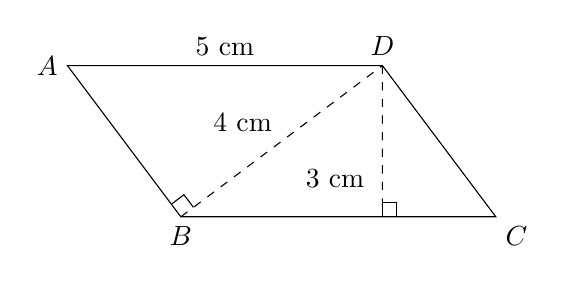
\begin{tikzpicture}[scale=.8]\coordinate(A)at(0,2.4);\coordinate(B)at(1.8,0);\coordinate(C)at(6.8,0);\coordinate(D)at(5,2.4);\draw(A)--(B)--(C)--(D)--cycle;\draw[dashed](B)--node[above left]{4 cm}(D);\draw[dashed](D)--node[pos=.75,left,xshift=-3pt]{3 cm}(5,0);\draw(5,0)rectangle(5.22,.22);\pic[draw,angle radius=2mm]{right angle=A--B--D};\node[above]at(2.5,2.4){5 cm};\node[left]at(A){$A$};\node[below]at(B){$B$};\node[below right]at(C){$C$};\node[above]at(D){$D$};\end{tikzpicture}

\end{document}
